\documentclass[9pt]{article}
\usepackage{a4wide}
\usepackage{graphicx}

\begin{document}

\section{Tage datafile description}

This file describes tage input files which describes whole scene.

\section{Comments}

The input file uses standard C++ comments:
\begin{verbatim}
// One line comment

/*
  Two or more line comment
*/
\end{verbatim}

\section{Properties}

All properties are set by
\begin{verbatim}
property_name = value
\end{verbatim}
a "value" can be strings, numbers (hexa, integer, float-point), colors, vectors
and enumerated values.

\subsection{Boolean}

Boolean is a binary value (true/false) and it's used for switches
or on/off properties. The false value is written as 0 and true any other
number (typically 1).
\begin{verbatim}
// light is enabled 
enable_ligth = 1

// shadows are disabled
enable_shadows = 0
\end{verbatim}

\subsection{Numbers}

Numbers are standard numerical values and can have a decimal part.
\begin{verbatim}
size = 10
height = 1.1
\end{verbatim}

\subsection{Strings}

Strings don't use commas and can't contain spaces. String values are typically 
used for modificator/generator names.
\begin{verbatim}
name = my_modificator_name
\end{verbatim}

\subsection{Colors}
Colors can be defined by three ways - by separated RGB values (0-255),
by one hexadecimal digit (HTML color) or as a vector (R,G,B). There is an example
of color\_center set to R:33, G:25, B:7
\begin{verbatim}
// by RGB:
color_center_r = 33
color_center_g = 25
color_center_b = 7

// by one hexa number (RRGGBB)
color_center = 211907

// by vector (R,G,B)
color_center = (33,25,7) 
\end{verbatim}
See the \_r,\_g and \_b suffixes. They are 0 by default.

\subsection{Vectors}

Vectors are composed from two or three numbers and they
can be integer or floating point numbers. For instance, we want to 
set light\_position vector:
\begin{verbatim}
light_position_x = -1
light_position_y =  1
light_position_z = -1
\end{verbatim}
See the \_x,\_y and \_z suffixes. They are 0 by default. Another option is
to use a vector format (x,y,z):
\begin{verbatim}
light_position = (-1,1,-1)
\end{verbatim}

\subsection{Angles}

An angles are normal numbers (an angle in degrees), from 0 to 360. 
They are used in polar coordinates and so on.
\begin{verbatim}
some_angle = 20.6
\end{verbatim}

\subsection{Enumerated types}

Enumerated types are values which can have some predefined values. 
They are typically used for blocks type descriptions, some types,
targets, operations and so on.
\begin{verbatim}
// coordinate type
type = MODIFICATOR_COORDINATE

// set modificator_target to texture
modificator_target = TEXTURE

// set modificator_target to geometry
modificator_target = GEOMETRY
\end{verbatim}

\subsubsection{Aritmetic operation}
It's one of frequently applied enumerated types and defines requested arithmetics
operation. It's used for coordinates, color/height operations and many more. Aritmetic 
operation anumerator is used in this context: 
\begin{verbatim}
result = destination OP source
\end{verbatim}
where OP is defined as: 
\begin{center}
\begin{tabular}{|l||l|}
SET & result = source\\
ADD & result = destination + source\\
SUB & result = destination - source\\
MODULATE & result = destination * source\\
MODULATE2X & result = destination * source * 2\\
\end{tabular}
\end{center}

\subsection{Intervals}
Some values can be set as interval. If a value is an interval,
it means it can get any value from the border values. The border values
are marked as "\_min" and "\_max" suffixes. Intervals are always used
with other types (number, angle, color, vector). Intervals can be set 
as a normal (non-interval) value, too.
\begin{verbatim}
/* Number intervals
*/
// Interval set by only one value so it's always 10
angle = 10

// Interval set by two border values, 
// can be any value from 10 to 20
angle_min = 10
angle_max = 20 

/* Vector intervals
*/ 
// As components
position_min_x = 10
position_min_y = 10
position_min_z = 10

position_max_x = 20
position_max_y = 20
position_max_z = 20

// As vectors
position_min = (10,10,10)
position_max = (20,20,20)

/* Color intervals
*/
// As components
color_min_r = 10
color_min_g = 10
color_min_b = 10

color_max_r = 20
color_max_g = 20
color_max_b = 20

// As vectors
color_min = (10,10,10)
color_max = (20,20,20)

// As hexadecimal (HTML) colors
color_min = 0a0a0a
color_max = 141414 
\end{verbatim}

\subsection{Coordinates}
Coordinates are 2D area which describes 
where a modificator is applied. The coordinate is a whole 
block with "type = MODIFICATOR\_COORDINATE", index (will be described later)
and start and size (or end) 2D vectors. There is an example of area
which starts at (0,0) and is 40x40 pixels wide:
\begin{verbatim}
{
  type = MODIFICATOR_COORDINATE

  index = 0

  start_x = 0
  start_y = 0

  size_x = 40
  size_y = 40
}
\end{verbatim}

\section{Basic blocks}
An atomic part of the file is a block inside compound braces. It describes one 
atomic unit inside generator or some generator values. Each block must
contain its name and type.
\begin{verbatim}
{
  name = generator
  type = GENERATOR_MESH

  /* All generator params come here
  */
}
\end{verbatim}
Blocks can be nested, like this one:
\begin{verbatim}
/* Describes pixel generator and its color definition
*/
{
  name = pixel_point
  type = MODIFICATOR_POINT_SINGLE

  {
    type = MODIFICATOR_POINT_SINGLE_COLOR
    color_center = 3b5528
  }
}
\end{verbatim}
All block examples bellow uses this format:
\begin{verbatim}
{
  /* First part contains block name and type:
  */
  name = block_name
  type = block_type

  /*
    Second part is a list of all posible properties,
    descriptions and default values:

    [property_type]  property_name
   
    If the property_type is an enumerated type, all 
    posibilies come here:
    
    VALUE_1
    VALUE_2
    VALUE_3
  */  
  property_name = default_value_of_the_property  
}
\end{verbatim}

\section{Generator architecture}
Whole generator is designed as a modificator chain. There is one master (root)
modificator and it passes results to slave modificators. A last modificator 
in the chain writes results (color pixel, heights) directly to a generator target
(it can be mesh itself, mesh texture or something else).

\clearpage

\begin{figure}[h]
\begin{center}
  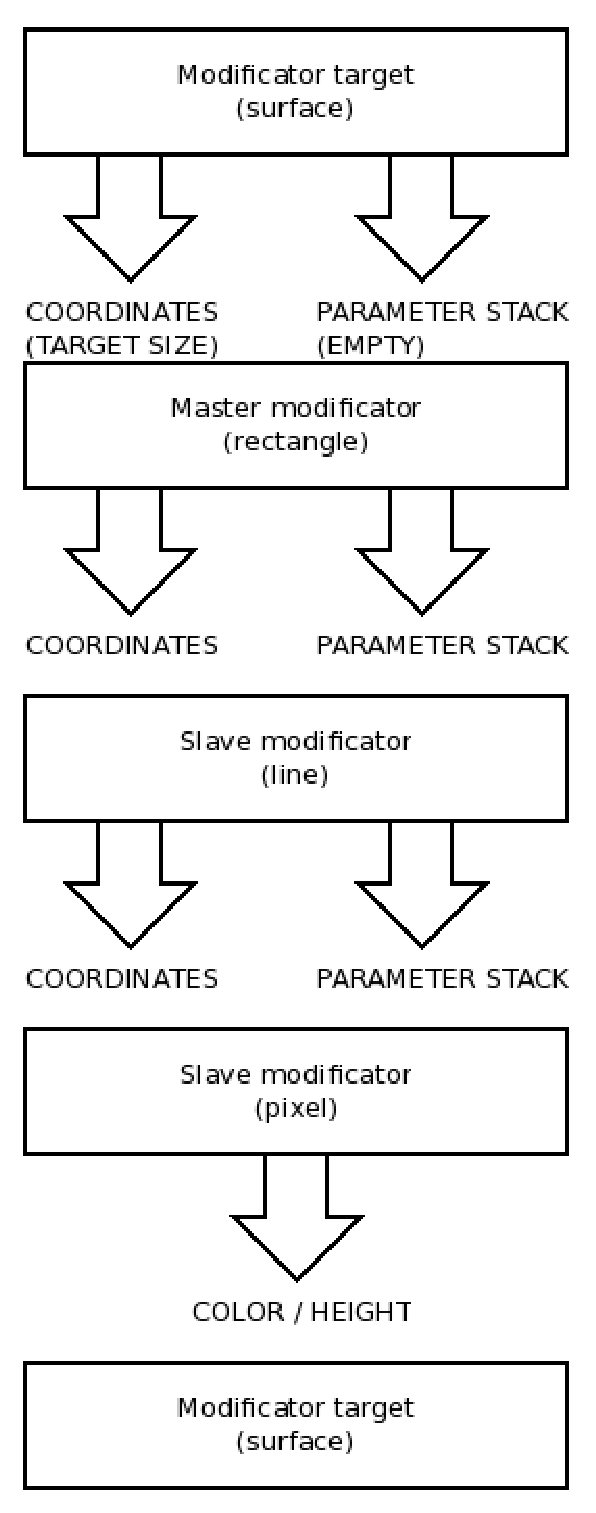
\includegraphics[scale=0.6]{p08.eps}
  \caption{Modificator chain which draws a line composed from single pixels.}
  \label{rect_line_example}
\end{center}
\end{figure}

A picture \ref{rect_line_example} is a nice example of a modificator chain. The first
modificator here is the rectangle and it's applied to whole
target surface because local coordinates are not defined. If the target surface
is 2048 pixels wide and 1024 pixels high, the rectangle will get \begin{math}(0,0) 
-> (2048, 1024)\end{math} coordinates. 

By default the rectangle modificator paints whole area by pixels. So it calls
specified slave modificator (the line here) for each pixel inside the \begin{math}(0,0) 
-> (2048, 1024)\end{math} target surface area.

A next modificator here is the line and it's drawn for each pixel inside the
target surface. We can define (by coordinate block inside the line modificator) the line
size and direction so we can obtain a rectangle filled by single lines. 
The lines are composed from single pixels which are drawn by 
the last modificator here - pixel.

\begin{itemize}
\item{\bf Modificators} are atomic generator parts specialized to one task. 
Each modificator is configured by properties (from the data file), 
coordinates (from the data file and/or previous modificator) and 
parameters (from previous modificator) and pastes its results 
(coordinates, properties, parameters) to another modificator.

For instance there is a modificator which generates a line and it 
pastes the results (coordinates for each single point which lies on the line) 
to another modificator which draws them.

\item{\bf Targets} are "final" modificators which transforms 
results into geometry (mesh) or texture. 

\item{\bf Generator} launches one or more modificators and 
specify which targets are used. An output of generator is 
a complete 3D object with material and texture. 

Generator itself can be used as a modificator so
if we take the line modificator from previous example, 
the line modificator \begin{math}->\end{math} pixel modificator \begin{math}->\end{math} 
texture target chain will generate single pixels to texture, but line modificator 
\begin{math}->\end{math} generator chain will generate complete 3D objects on given coordinates.

\item{\bf Generator launcher} launches generators.

\end{itemize}

\section{Generators}

\subsection{Generator launcher}
Generator launcher defines which generators are performed and their order. 
It can be only one in the whole data file.
\begin{verbatim}
{
  /* Launcher name and type
  */
  name = generator_launcher_name
  type = GENERATOR_LAUNCHER

  /* Performed generators. 
  */
  generator_mesh = first_generator
  generator_mesh = second_generator
  generator_mesh = third_generator
}
\end{verbatim}

\subsection{Generator}
Generator defines which modifiators are launched, their targets and order. 
There can be as many generators as you want in a data file and 
are distinguished by their names:
\begin{verbatim}
/* A simple generator
*/
{
  /* Generator name and type
  */
  name = generator_name
  type = GENERATOR_MESH

  /*
    Modificator name and its target:
    
    [string]          modificator
    [enumerated type] modificator_target
      
      TEXTURE
      GEOMETRY
      GENERATOR_MESH
      AUX
  */
}
\end{verbatim}
\subsubsection*{Generator items}
\begin{itemize}
\item{\bf modificator} - launches a generators with this name.
\item{\bf modificator\_target} - defines a target of the generator.
\begin{itemize}
\item{\bf TEXTURE} - texture target (color or height)
\item{\bf GEOMETRY} - heights in mesh geometry
\item{\bf GENERATOR\_MESH} - target is another generator
\item{\bf AUX} - an auxiliary surface (color or height)
\end{itemize}
\end{itemize}
There is an example of a generator there:
\begin{verbatim}
/* A simple generator
*/
{
  /* Generator name and type
  */
  name = generator_name
  type = GENERATOR_MESH
  
  /* First modificator name and its target
  */
  modificator = first_modificator
  modificator_target = TEXTURE
  
  /* Second modificator name and its target
  */
  modificator = second_modificator
  modificator_target = GEOMETRY
}
\end{verbatim}

\subsection{Generated object parameters}
A 3D object generated by single generator is (for now) a flat mesh with
one big texture. If the texture is too big, it's sliced to smaller parts.
The object is described by mesh, material and texture block.

\subsubsection{Mesh params}
Describes generated mesh parameters like type, size and so on:
\begin{verbatim}
{
  name = mesh_name
  type = MESH_PARAMS

  /*
    [enumerated value]  mesh_type
   
      MESH_LAND
      MESH_BUNCH
      MESH_GRASS
      MESH_BUSH
  */
  mesh_type = MESH_LAND
  
  /*
    Mesh dimensions. All values are vectors.
  
    [vector] start
    [vector] diff
    [vector] size
  */  
  start = (0,0,0)
  diff = (1,1,1)
  size = (1,1,1)
  
  /*
    Parameters related to bunch:
    
    [int, interval]   bunch_slice_num
    [int, interval]   bunch_slice_segments
      
    [float, interval] bunch_slice_x_offset
    [float, interval] bunch_slice_z_offset
      
    [angle, interval] bunch_slice_falling
    [angle, interval] bunch_segment_falling
        
    [int]             bunch_slice_rotation_incemental
    [angle, interval] bunch_slice_rotation_range
    [angle, interval] bunch_slice_rotation_step
  */    
  bunch_slice_num = 6
  bunch_slice_segments = 1
  
  bunch_slice_x_offset = 0
  bunch_slice_z_offset = 0
  
  bunch_slice_falling = 0
  bunch_segment_falling = 0
  
  bunch_slice_rotation_incemental = 0
  bunch_slice_rotation_range = 180
  bunch_slice_rotation_step = 0
}
\end{verbatim}
\subsubsection*{Mesh items}
\begin{itemize}
\item{\bf mesh\_type} - 
\begin{itemize}
\item{\bf MESH\_LAND} - a flat land
\item{\bf MESH\_BUNCH} - a bunch of plates
\item{\bf MESH\_GRASS} - not implemented yet
\item{\bf MESH\_BUSH} - not implemented yet
\end{itemize}
\item{\bf start} - mesh location
\item{\bf diff} - a size of one segment
\item{\bf size} - number of segments
\item{\bf bunch\_slice\_num}
\item{\bf bunch\_slice\_segments}
\item{\bf bunch\_slice\_x\_offset}
\item{\bf bunch\_slice\_z\_offset}
\item{\bf bunch\_slice\_falling}
\item{\bf bunch\_segment\_falling}
\item{\bf bunch\_slice\_rotation\_incemental}
\item{\bf bunch\_slice\_rotation\_range}
\item{\bf bunch\_slice\_rotation\_step}
\end{itemize}

\subsubsection{Material params}
Describes material of a generated mesh:
\begin{verbatim}
{
  name = test_material
  type = MATERIAL_PARAMS
  
  /*
    [boolean] transparent
    [boolean] double_side
  */
  transparent = 0
  double_side = 0  
}
\end{verbatim}
\subsubsection*{Material items}
\begin{itemize}
\item{\bf transparent} - transparent material are for bunches
\item{\bf double\_side} - double sided material are used by bunches
\end{itemize}

\subsubsection{Texture params}
Describes texture for a generated mesh.
\begin{verbatim}
{
  name = test_texture
  type = TEXTURE_PARAMS

  /*
    [vector]  texture_size
    [int]     texture_height
    [color]   background_color
    [int]     texture_alpha
  */
  texture_size = (512,512)  
  texture_height = 512
  background_color = (0,0,0)
  texture_alpha = 0
}
\end{verbatim}
\subsubsection*{Texture items}
\begin{itemize}
\item{\bf texture\_size}
\item{\bf texture\_height}
\item{\bf background\_color}
\item{\bf texture\_alpha}
\end{itemize}

\section{Generator targets}
\subsection{GEOMETRY target}
\subsection{TEXTURE target}
\subsection{GENERATOR\_MESH target}
\subsection{AUX target}

\section{Generator modificators}

\subsection{A generic modificator}
There is a basic setup which is included in any modificator.
All properties are available in all modificators,
although they do not have to implement all of them
and some properties can have a different meaning.
\begin{verbatim}
{
  /*
    Basic modificator properties:
  
    [boolean] area_inverted
    [int]     pixel_size
    
    [int]     pixel_step
    [int]     pixel_step_x
    [int]     pixel_step_y
  
    [boolean] pixel_step_random
    [int]     pixel_step_random_min
    [int]     pixel_step_random_max
    
    [float]   pixel_color_density
    
    [boolean] probability_fade
    [float]   probability_fade_start
    [float]   probability_fade_stop
  
    [boolean] color_fade
    [float]   color_fade_start
    [float]   color_fade_stop
      
    [boolean] erode_border
    [float]   erode_factor
    
    [float]   size_variator_theshold
    [float]   size_variator_factor
  */    
    
  /*
    Mask properties:
    
    [string]  mask
  */
    
  /*
    Slave modificators:
  
    [string] modificator_slave
    [string] modificator_pre
    [string] modificator_post
  */  

  /*
    Local coordinates
    
    Each basic setup may contain local coordinate setup. It's defined by nested 
    MODIFICATOR_COORDINATE block and is described in next chaper.
  */
}
\end{verbatim}
\subsubsection*{Generic modificator properties}
\begin{itemize}
\item{\bf area\_inverted} - inverted rendering.
\item{\bf pixel\_size} - size of single pixel. It's used only by MODIFICATOR\_POINT\_SINGLE.
\item{\bf pixel\_step} - distance between pixels, draws grid instead of solid surface.
\item{\bf pixel\_step\_x} - distance between pixels in X asis.
\item{\bf pixel\_step\_y} - distance between pixels in Y asis.
\item{\bf pixel\_step\_random} - randomize pixel distances.
\item{\bf pixel\_step\_random\_min, pixel\_step\_random\_max} - pixel distance boundary. 
\item{\bf pixel\_color\_density} - a probability of pixel emission, from
\begin{math}<0,1>\end{math} range.
\item{\bf probability\_fade} - pixel probability fading, it's used by MODIFICATOR\_POINT\_EXTENDED only.
\item{\bf probability\_fade\_start}
\item{\bf probability\_fade\_stop}
\item{\bf color\_fade} - pixel color fading, it's used by MODIFICATOR\_POINT\_EXTENDED only.
\item{\bf color\_fade\_start}
\item{\bf color\_fade\_stop}
\item{\bf erode\_border} - pixel border erosion.
\item{\bf erode\_factor}
\item{\bf size\_variator\_theshold} - obsolete.
\item{\bf size\_variator\_factor} - obsolete.
\item{\bf mask}
\end{itemize}
\begin{itemize}
\item{\bf modificator\_slave} - it's called for each coordinate generated 
by this master modificator.
\item{\bf modificator\_pre} - it's called before modificator start 
and with top coordinates only.
\item{\bf modificator\_post} - it's called when modificator finishes 
and with top coordinates only.
\end{itemize}
As for slave modificators - you can define up to five slave modificators for each class.
Those modificators are called in order how is defined.

\subsection{Coordinates}
Each modificator is applied to an area which is restricted by "top" coordinates. 
Top coortinates are defined by master modificator or size of target surface 
for the first modificator.

\begin{figure}[h]
\begin{center}
  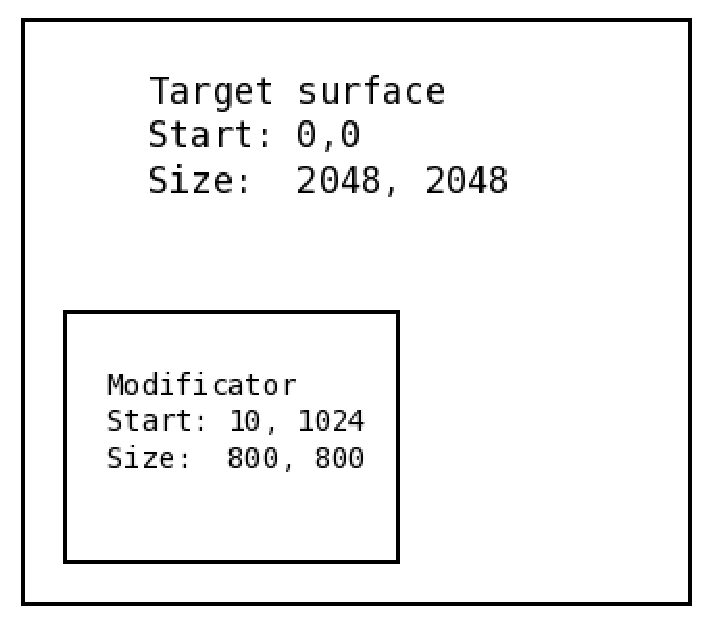
\includegraphics[scale=0.6]{p02.eps}
  \caption{Target surface and one modificator.}
\end{center}
\end{figure}

Those "top" coordinates are further modified by local
coordinate block (randomization, size extension
and so on).

\subsection{Coordinate block}
Defines a block with {\bf local} coordinate configuration. 
Top coordinates are defined by master modificator or modificator target and
local coordinates are defined by coordinate block which can be included in
any modificator.

\begin{figure}[h]
\begin{center}
  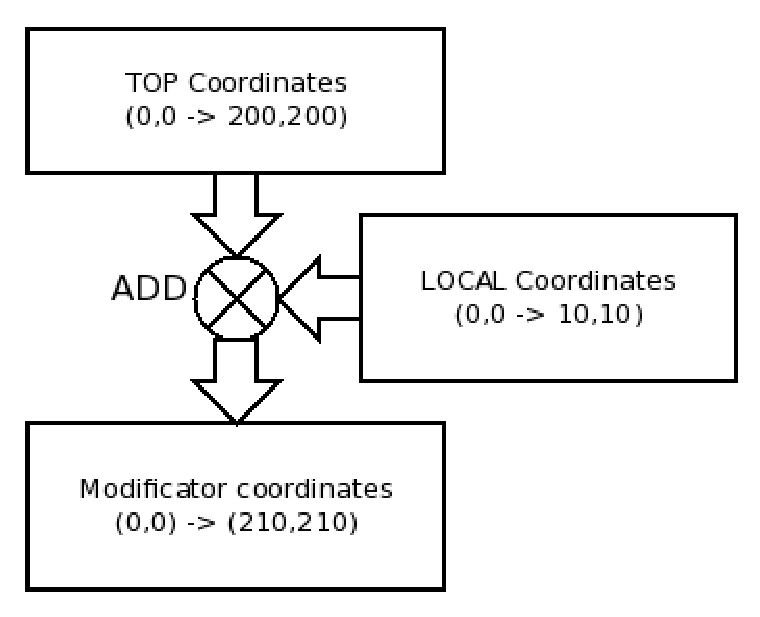
\includegraphics[scale=0.6]{p06.eps}
  \caption{An example of top and local coordinates composition.}
\end{center}
\end{figure}

Coordinate block defines operation between top and local coordinates, whether the local
ones are generated (randomized) or not and so forth. If there are more than one
coordinate block, the modificator is called for each of them.

\subsubsection*{Coordinate setup properties}
\begin{verbatim}
{
  /*
    Local coordinates setup:
    
    [aritmetic operation] coordinates_operation 
    [boolean]             coordinates_random
    [int]                 coordinates_random_num
    [enumerated type]     modificator_start
    [enumerated type]     modificator_size
            
      COORD_CURRENT
      COORD_LAST_START
      COORD_LAST_SIZE
      COORD_LAST_START_SIZE      
  */  
  coordinates_operation = OPERATION_SET
  coordinates_random = 0
  coordinates_random_num = 0
  modificator_start = COORD_CURRENT
  modificator_size = COORD_CURRENT
  
  /*
    First coordinates blocks:
  */
  {
    type = MODIFICATOR_COORDINATE
    
    /*
      [vector] start
      [vector] size
      [int]    index
    */
  }
  
  /*
    Second coordinates blocks:
  */
  {
    type = MODIFICATOR_COORDINATE
    
    /*
      [vector] start
      [vector] size
      [int]    index
    */
  }
  
  /*
    Third one...
  */
  {
    [...]
  }
}
\end{verbatim}
\subsubsection*{Coordinate block properties}
\begin{itemize}
\item{\bf coordinates\_operation} - defines operation between top and local coordinates.
\item{\bf coordinates\_random} - if it's set to 1, local coordinates are generated by random number
generator in boundaries given by coordinates with index 0 and index 1 (see bellow).
\item{\bf coordinates\_random\_num} - number of generated local coordinates.    
\item{\bf modificator\_start, modificator\_size} - it defines parts of top 
coordinates (start and size parts) for current coordinates\_operation. 
It can be top coordinates from previous modificator (COORD\_CURRENT) or 
result of last top and local coordinates composition:
\begin{itemize}
\item{\bf COORD\_CURRENT} - current top coordinates
\item{\bf COORD\_LAST\_START} - start of last coordinate composition (start part)
\item{\bf COORD\_LAST\_SIZE} - size of last coordinate composition (size part)
\item{\bf COORD\_LAST\_START\_SIZE} - endpoint of last coordinate composition (start+size parts).
It's userful for generating objects which have to be connected (e.g. objects strips).
\end{itemize}
\end{itemize}
\subsubsection*{Modificator coordinate sub-block properties}
\begin{itemize}
\item{\bf start} - coordinate start
\item{\bf size} - coordinate size, endpoint is calculated as start+size
\item{\bf index} - coordinate index (used by randomized local coordinates, see bellow)
\end{itemize}

\begin{figure}[h]
\begin{center}
  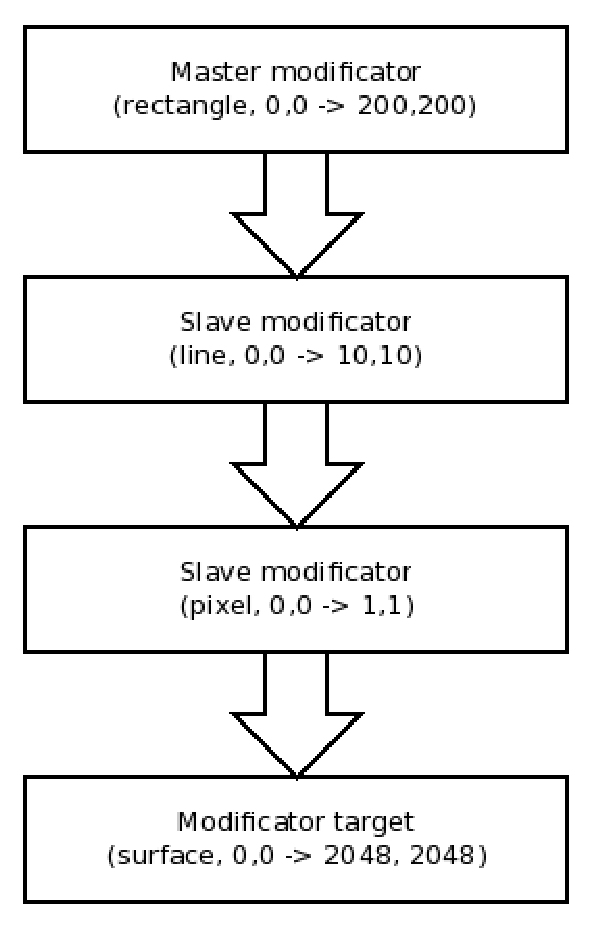
\includegraphics[scale=0.6]{p05.eps}
  \caption{An example of modificator chain with local coordinate setup.}
\end{center}
\end{figure}

\subsection{Modificator parameters}

Parameters are float point values in \begin{math}<0,1>\end{math} range which are passed between
modificators on parameter stack. If a modificator generates any parameter, the
parameter is added on top of the parameter stack. If a modificator does not
emit any parameter the stack is passed without modification.

The parameters and are typically used by simple point modificator 
for color/height generation and so on. For instance, there's a fractal
modificator which generates a height map. The fractal modificator calls
a slave modificator (simple point modificator for instance) for each generated 
pixel and as parameter passes pixel height. So the slave pixel modificator can 
draw pixels by color adjusted by pixel height. Another example showns 
figure \ref{rect_line_example}.

\subsubsection*{Modificator parameters type}

Modificator parameters are defined by modificator parameter enum type:
\begin{center}
\begin{tabular}{|l||l|}
PARAM\_PREV\_0 & a parameter on top of the parameter stack \\
PARAM\_PREV\_1 & a second one \\
PARAM\_PREV\_2 & third... \\
PARAM\_PREV\_3 & \\
PARAM\_PREV\_4 & \\
PARAM\_SCATTER & a random number from \begin{math}<-1,1>\end{math} range \\
PARAM\_SCATTER\_HALF & a random number from \begin{math}<0,1>\end{math} range \\
PARAM\_HEIGHT\_MAP & not implemented yet \\
PARAM\_HEIGHT\_MESH & not implemented yet \\
DEFAULT & an alias for PARAM\_SCATTER\_HALF \\
\end{tabular}
\end{center}

\subsection{Point modificators}

Point modificators are designed as last modificators and usually write
data directly to targets (height to mesh geometry or color/heights to texture). 

\subsubsection{Single point modificator}

Single point modificator writes to target (slave modificator
or texture target) only one single point. Its size is always 1x1 so for instance
if it gets \begin{math}(20,20) -> (100,100)\end{math} coordinate 
from master modificator, it writes only single pixel to \begin{math}(20,20)\end{math} 
with \begin{math}(1,1)\end{math} size. Pixel\_size property is ignored 
by this modificator.

The single point modificator consists from basic setup in main block and
subblocks. The subblocks define particular color/height operations and 
are subsequently applied to a temporary color/height value. Number of 
color/height subblocks is not limited.

This temporary color is get from modificator target, goes through subblocks
and is applied back to modificator target (as color/height to texture or
height to mesh geometry). 

\subsubsection*{Single point modificator block contains}
\begin{verbatim}
{
  name = some_modificator_name
  type = MODIFICATOR_POINT_SINGLE

  /*    
    Generator type:
  
    [enumerated type]  generator_type
            
      GENERATOR_GAUSS
      GENERATOR_RAND
      
    [boolean]          generator_separated     
  */
  generator_type = GENERATOR_GAUSS
  generator_separated = 0
    
  /*
    Color operations:
    
    [aritmetic operation]  color_operation        
    [bool]                 color_blend
  */      
  color_operation = SET
  color_blend = 0
  
  /*
    Height operation:
    
    [aritmetic operation]  height_operation
   */
  height_operation = SET

  /*
    Generated colors can be crop:
  
    [boolean]               color_borders
    [color]                 color_border_min
    [color]                 color_border_max
   */
  color_borders = 0
  color_border_min = (0,0,0)
  color_border_max = (255,255,255)
  
  /*
    Color tables:
          
    [string]                color_table
    [string]                color_table_center
    [string]                color_table_delta    
  */
  
  /*
    Color subblock describes single color operation.
  */
  {
    type = MODIFICATOR_POINT_SINGLE_COLOR
    [...]
  }
  
  /*
    Height subblock describes single height operation.
  */
  {
    type = MODIFICATOR_POINT_SINGLE_HEIGHT
    [...]
  }
}
\end{verbatim}
\subsubsection*{Single point modificator properties}
\begin{itemize}
\item{\bf generator\_type} - it's a generator type used for PARAM\_SCATTER 
and PARAM\_SCATTER\_HALF randomisation.
\begin{itemize}
\item{\bf GENERATOR\_GAUSS}
\item{\bf GENERATOR\_RAND}
\end{itemize}
\item{\bf generator\_separated} - for each cycle in color/height box (see bellow) is
generated a new random value
\item{\bf color\_operation} - color operation between target and color pixels 
generated by this modificator
\item{\bf color\_blend} - blend the generated pixels
\item{\bf height\_operation} - height operation between target and heights
generated by this modificator
\item{\bf color\_borders} - are generated colors shrink to this range?
\item{\bf color\_border\_min} - minimal border color
\item{\bf color\_border\_max} - maximal border color
\end{itemize}
Color table can define a colors which can be used for color generation. 
For instance you can take a picture and generate pixels with colors from
the image. If the color table is active, for each generated
color is located the nearest color in the image (in RGB) and the nearest 
color is used as a result instead of the generated one.
\begin{itemize}
\item{\bf color\_table} - Image file (png, jpg,...) witch will be used for 
color table composition. Final generated colors are altered with colors from this table.
\item{\bf color\_table\_center} - Image file (png, jpg,...) witch will be used 
for color table composition. Center colors (from each color box) are altered 
with colors from this table.
\item{\bf color\_table\_delta} - Image file (png, jpg,...) witch will be used 
for color table composition. Delta colors (from each color box) are altered 
with colors from this table.
\end{itemize}

\subsubsection*{Generated parameters}

None.

\subsubsection{Single point modificator - color subblock}

Color subblocks defines a single color operation and a result
is a single color which is applied to a temporary color. The temporary color
is loaded from target surface and when all color blocks are 
processed it's written back to target surface.

\begin{figure}[h]
\begin{center}
  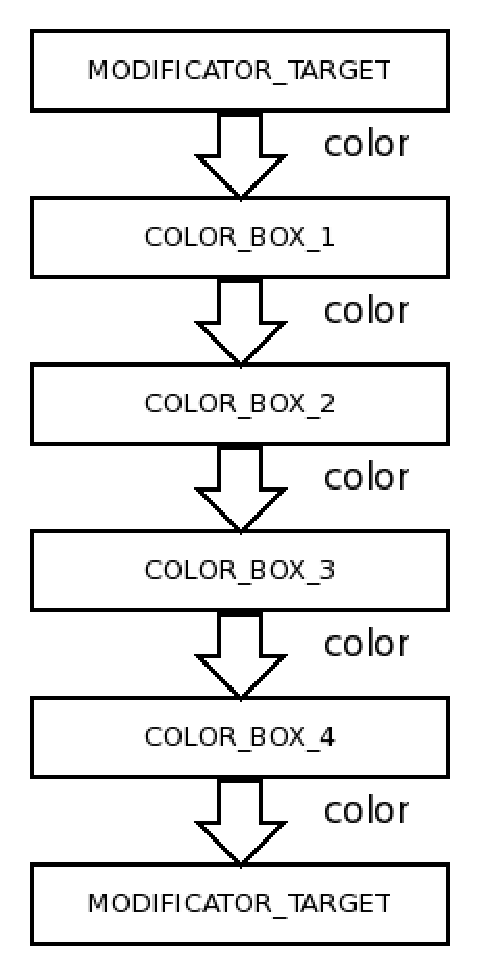
\includegraphics[scale=0.6]{p04.eps}
  \caption{Color sub-block workflow.}
  \label{color_sub_block_workflow}
\end{center}
\end{figure}

\subsubsection*{Color subblock scheme}

The color subblock is applied to input color
and passes the result as an output color. The color operation 
applied to the input color is contoled by another input - 
a modifiator parameter. This parameter can be a random number, a parameter
from previous modifiator and so on (see {\bf Modificator parameters} chaper).

\begin{figure}[h]
\begin{center}
  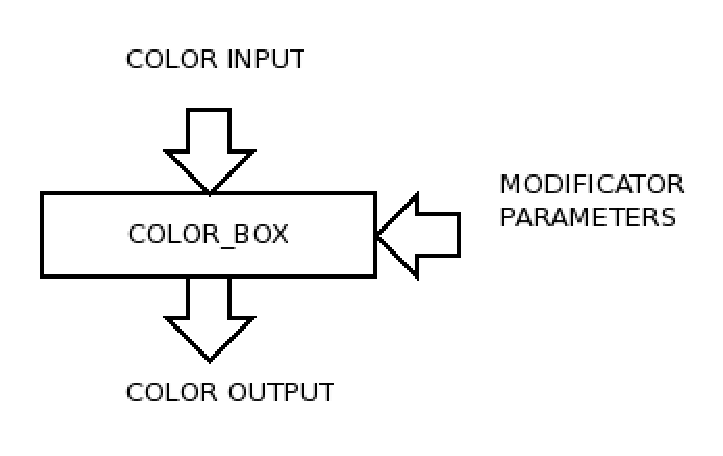
\includegraphics[scale=0.6]{p07.eps}
  \caption{Color sub-block flow.}
  \label{color_sub_block_flow}
\end{center}
\end{figure}

\subsubsection*{Color output calculation}

There is a figure \ref{color_output_calculation} with detailed schema 
how the color subblock output is calculated. There are two main components - 
{\bf COLOR\_DELTA} which is directly defined in the block and 
{\bf COLOR\_CENTER\_CURRENT} which will be described later.

The {\bf COLOR\_DELTA} parameter is scaled by {\bf COLOR\_DELTA\_SCALE} 
and then by modifiator parameter defined by {\bf color\_delta\_parameter}. 
A color operation defined by {\bf color\_operation} is calculated 
and a result of this is combined with input color (by {\bf final\_operation}).

This operation is executed for every pixel which is processed by 
this modificator.

\begin{figure}[h]
\begin{center}
  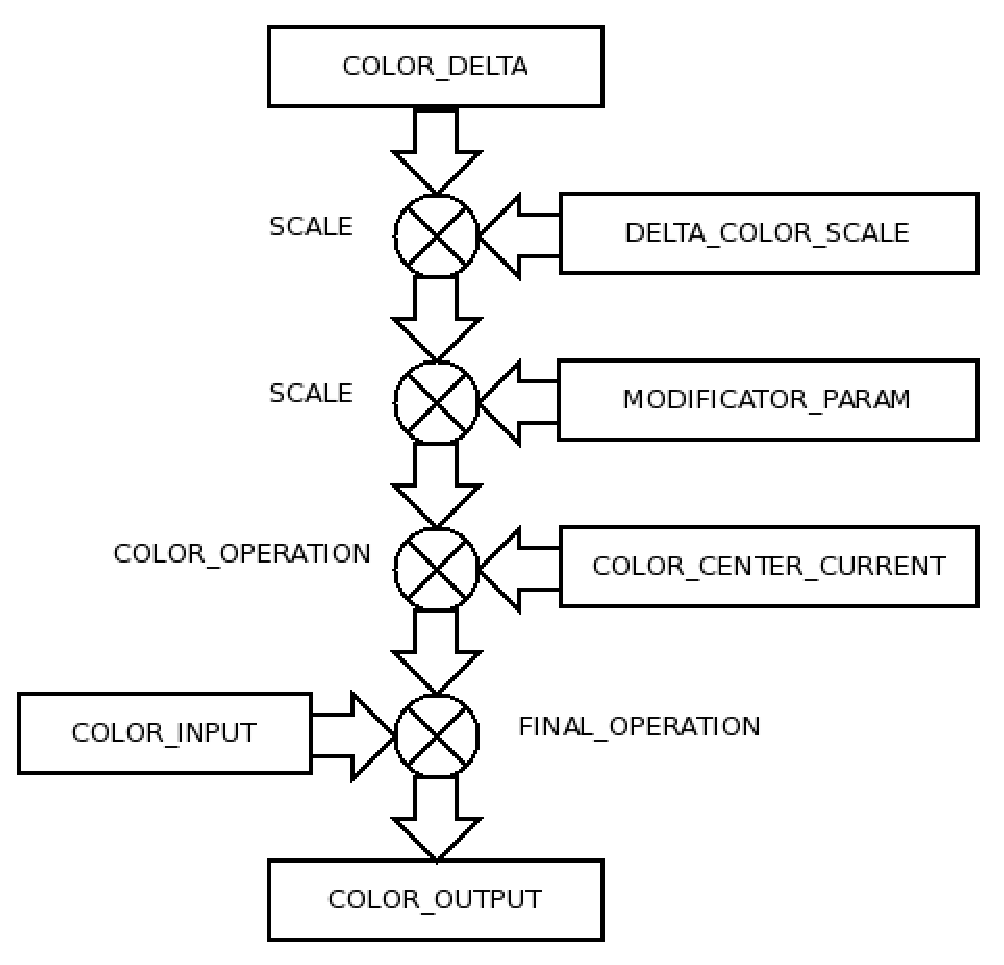
\includegraphics[scale=0.6]{p09.eps}
  \caption{Color output calculation.}
  \label{color_output_calculation}
\end{center}
\end{figure}

\subsubsection*{Color center current calculation}

{\bf COLOR\_CENTER\_CURRENT} which is referenced in previous paragraph is 
calculated only once before the pixels are emitted and then remains constant. 
It's useful when you want to set a background color whith some
variation.

\begin{figure}[h]
\begin{center}
  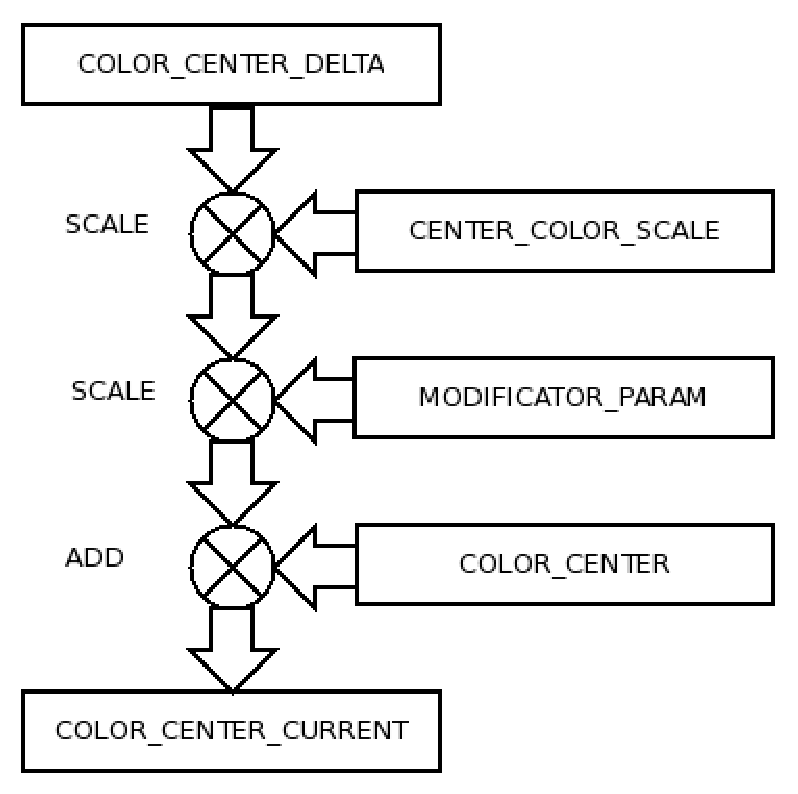
\includegraphics[scale=0.6]{p10.eps}
  \caption{Color center current calculation.}
  \label{color_center_current_calculation}
\end{center}
\end{figure}

\clearpage
\subsubsection*{Color subblock format}
\begin{verbatim}
{
  type = MODIFICATOR_POINT_SINGLE_COLOR

  /*  
    [aritmetic operation]   final_operation
    [boolean]               final_blend
    [modificator parameter] final_blend_parameter
  */
  final_operation = SET
  final_blend = 0
  final_blend_parameter = DEFAULT
  
  /*
    [aritmetic operation]   color_operation
    [boolean]               color_blend
    [modificator parameter] color_blend_parameter
  */
  color_operation = ADD
  color_blend = 0
  color_blend_parameter = DEFAULT
  
  /*
    [color]                 color_center
    [float]                 color_center_scale
    [float]                 color_center_delta
    [modificator parameter] color_center_parameter
  */
  color_center = (0,0,0,0)
  color_center_scale = 1
  color_center_delta = (0,0,0,0)
  color_center_parameter = PARAM_SCATTER_HALF;
  
  /*
    [color]                 color_delta
    [float]                 color_delta_scale
    [modificator parameter] color_delta_parameter
  */
  color_delta = (0,0,0,0)
  color_delta_scale = 1
  color_delta_parameter = PARAM_SCATTER_HALF
  
  /*
    Shortcuts for color definition:
    
    [color]                 color_min
    [color]                 color_max

    [color]                 color_center_min
    [color]                 color_center_max
  */  
}
\end{verbatim}
\subsubsection*{Color subblock properties}
Color operations:
\begin{itemize}
\item{\bf final\_operation} - a color operation between color input and 
current color block result.
\item{\bf final\_blend} - enable color blending for {\bf final\_operation}.
\item{\bf final\_blend\_parameter} - a parameter for {\bf final\_operation} blending.
\item{\bf color\_operation} - a color operation between current color center and
color delta.
\item{\bf color\_blend} - enable color blending for this operation.
\item{\bf color\_blend\_parameter} - a parameter used for this color blending.
\end{itemize}
{\bf COLOR\_CENTER\_CURRENT} calculation:
\begin{itemize}
\item{\bf color\_center}
\item{\bf color\_center\_scale}
\item{\bf color\_center\_delta}
\item{\bf color\_center\_parameter}
\end{itemize}
Parameters related to {\bf color\_operation}:
\begin{itemize}
\item{\bf color\_delta}
\item{\bf color\_delta\_scale}
\item{\bf color\_delta\_parameter}
\end{itemize}
Shortcuts for color definition:
\begin{itemize}
\item{\bf color\_min, color\_max} - a shortcut for color\_center and color\_delta
definition:
\begin{verbatim}
color_center = color_min
color_delta = (color_max-color_min)
\end{verbatim}
\item{\bf color\_center\_min, color\_center\_max} - a shortcut for color\_center
and color\_center\_delta definition:
\begin{verbatim}
color_center = color_center_min
color_center_delta = (color_center_max-color_center_min)
\end{verbatim}
\end{itemize}

\subsubsection{Single point modificator - height subblock}

Height subblock is similar to color subblock but
with float point numbers (from 0 to 1). Final height
is calculated as:
\begin{verbatim}
height_delta_tmp = height_delta * height_parameter
height_current = height_center (height_operation) height_delta_tmp;
height_output = height_input (final_operation) height_current;
\end{verbatim}
Where {\bf height\_input} is a height loaded from target surface or previous
block and {\bf height\_output} is a final result.

\subsubsection*{Height subblock structure}
\begin{verbatim}
{
  type = MODIFICATOR_POINT_SINGLE_HEIGHT

  /*    
    [float]                 height_center
    [float]                 height_delta
  */
  height_center = 0
  height_delta = 0

  /*
    [modificator parameter] height_parameter
  */  
  height_parameter = PARAM_SCATTER_HALF
  
  /*  
    [aritmetic operation]   height_operation
  */
  height_operation = ADD
  
  /*  
    [aritmetic operation]   final_operation
  */
  final_operation = SET
  
  /*
    [float]                 height_min
    [float]                 height_max    
  */  
}
\end{verbatim}
\subsubsection*{Height subblock properties}
\begin{itemize}
\item{\bf height\_center}
\item{\bf height\_delta}
\item{\bf height\_parameter}
\item{\bf height\_operation}
\item{\bf final\_operation}
\end{itemize}
Shortcuts for height definition:
\begin{itemize}
\item{\bf height\_min, height\_max} - it's a shortcut for {\bf height\_center} and 
{\bf height\_delta} definition.
\begin{verbatim}
height_center = height_min
height_delta = (height_max - height_min)
\end{verbatim}
\end{itemize}

\subsubsection{Extended point modificator}

Extended point modificator draws a point (circle)
from single pixels. The pixel generation is controlled by 
properties of generic (basic) modificator.
\begin{verbatim}
{
  name = some_modificator_name
  type = MODIFICATOR_POINT_EXTENDED
}
\end{verbatim}
\subsubsection*{Extended point modificator properties}
Extended point modificator does not have any specific properties.
\subsubsection*{Generated parameters}

None.

\subsection{Rectangle modificator}

Rectangle modificator generates points in whole area defined by coordinates.
\begin{verbatim}
{
  name = some_modificator_name
  type = MODIFICATOR_RECT
}
\end{verbatim}
\subsubsection*{Rectangle modificator properties}
Extended point modificator does not have any specific properties.
\subsubsection*{Generated parameters}

None.

\subsection{Height modificators}

Heightmap modifiators are used for height or parameter generation.

\subsubsection{Height map modificator}

Heightmap modifiator is a simple heigtmap which can be loaded from a bitmap
file, a target surface or generated by a fractal generator. Its typically useful
as a master modificator for MODIFICATOR\_POINT\_SINGLE, where pixel height
is inserted to parameter stack, passed to MODIFICATOR\_POINT\_SINGLE modifiator
and used for color shift there.

\begin{verbatim}
{
  name = some_modificator_name
  type = MODIFICATOR_HEIGHT_MAP
  
  /*    
    [string]    height_bitmap
    [string]    height_source
  */
  
  /*
    [boolean]   heightmap_intensity
  */
  heightmap_intensity = 1
  
  /*    
    [float]     height_multiplier
    [float]     height_shift
  */
  height_multiplier = 1
  height_shift = 0
  
  /*
    [float]     height_range_min
    [float]     height_range_max
  */  
  height_range_min = 0
  height_range_max = 1
  
  /*  
    [boolean]   scale_target
    [int]       scale_width
    [int]       scale_height
  */
  heightmap_scale = 0
  height_scale_width = 0
  height_scale_height = 0
}
\end{verbatim}
\subsubsection*{Height map modificator properties}
\begin{itemize}
\item{\bf height\_bitmap} - Image file (png, jpg,...) witch will be used as 
source for heigtmap, where height is computed from color intensity.
\item{\bf height\_source} - a name of modifiator where the heightmap is obtained from.
\item{\bf heightmap\_intensity} - calculate illumination for each pixel an pass it
to parameter stack.
\item{\bf height\_multiplier, height\_shift} - pixel height modificators:
\begin{verbatim}
height_final = height_pixel * height_multiplier + height_shift
\end{verbatim}
\item{\bf height\_range\_min, height\_range\_max} - height range filter. Pixels
outside this range are ignored.
\item{\bf scale\_target}
\item{\bf scale\_width}
\item{\bf scale\_height}
\end{itemize}

\subsubsection*{Generated parameters}
\begin{tabular}{|l||l|}
  Parameter & Meaning \\
  0 & relative pixel height \\
  1 & pixel height \\
  2 & pixel intensity \\
\end{tabular}

\paragraph*{Relative pixel height}
means that pixel height is clamped to \begin{math}{\bf<height\_range\_min, height\_range\_max>}\end{math}
ranges and adjusted by {\bf height\_multiplier} and {\bf height\_shift}.
The formula is:
\begin{verbatim}
height_translated = (height_pixel - height_range_min) / (height_range_max - height_range_min)
height_output = height_translated*height_multiplier + height_shift
\end{verbatim}

\paragraph*{Pixel height} is an absolute pixel height. 
If {\bf height\_range\_min = 0.5} and {\bf height\_range\_max = 0.8},
all pixels are at this range \begin{math}<0.5,0.8>\end{math}.

\paragraph*{Pixel intensity} means that a normal vector is 
calculated and its dot-product with light vector 
is passed here. The light vector is (0,1,0) by default.

\subsubsection{Mid-point modificator}

Mid point fractal generator is derived from heightmap modificator
so its result is a heighmap. An output of fractal generator is written to 
temporary heighmap modificator, normalized to \begin{math}<0,1>\end{math} 
range and processed as a normal heighmap, so all properties of heightmap 
modificator can be used.

\begin{verbatim}
{
  name = some_modificator_name
  type = MODIFICATOR_FRACTAL

  /*
    [float]             fractal_hurst
  */
  generator_hurst = 0.6
  
  /*
    [float]             fractal_delta
    [float]             fractal_center
  */
  fractal_delta = 1
  fractal_center = 0
  
  /*
    [int]               limited_iteration
    [float]             limited_iteration_value
    
    [float]             correction_center
    [float]             correction_border
    
    [int]               filter_back
    [float]             border_start
    [float]             perturbation
    
    [int]               pixel_fill
    [int]               pixel_distance
    
    [int]               pixel_filter
    [int]               pixel_filter_num
  
    [enumerated type]   interpolation
      MID_POINT
      LINE_MIN
      LINE_MAX
      LINE_CENTER
      LINE_PRIORITY_HIGH
      LINE_PRIORITY_LOW
      LINE_RANGE_HIGH
      LINE_RANGE_LOW
      LINE_RANDOM
      
    [enumerated type]   interpolation_first
      MID_POINT
      LINE_MIN
      LINE_MAX
      LINE_CENTER
      LINE_PRIORITY_HIGH
      LINE_PRIORITY_LOW
      LINE_RANGE_HIGH
      LINE_RANGE_LOW
      LINE_RANDOM

    [enumerated type]   interpolation_second
      MID_POINT
      LINE_MIN
      LINE_MAX
      LINE_CENTER
      LINE_PRIORITY_HIGH
      LINE_PRIORITY_LOW
      LINE_RANGE_HIGH
      LINE_RANGE_LOW
      LINE_RANDOM
        
    [int]               interpolation_border      
    [int]               generation_border
  */  
}
\end{verbatim}
\subsubsection*{Mid-point modificator properties}
\begin{itemize}
\item{\bf fractal\_hurst} - A hurst coeficient for fractal generator. Low value 
(around 0.2) means great height variation, high values (around 0.8) produces soft shapes.
\item{\bf fractal\_delta, fractal\_center} - An output height is produced as
\begin{verbatim}
height_output = fractal_delta * height_generated + fractal_center;
\end{verbatim}
\item{\bf limited\_iteration} - By default the hight values are emitted for all pixels
inside the coordinate area. By limited\_iteration you can enable restrictions 
for total iterations number.
\item{\bf limited\_iteration\_value} - Maximal number of iterations.
\item{\bf correction\_center}
\item{\bf correction\_border}
\item{\bf filter\_back}
\item{\bf border\_start}
\item{\bf perturbation}
\item{\bf pixel\_fill}
\item{\bf pixel\_distance}
\item{\bf pixel\_filter}
\item{\bf pixel\_filter\_num}
\item{\bf interpolation} - A new height values are derived
from their four neighbor points and you can define how the new value is calculated
and which points are processed. 
\begin{itemize}
\item{\bf MID\_POINT} - An averange value of all four points is used.
\item{\bf LINE\_MIN}
\item{\bf LINE\_MAX}
\item{\bf LINE\_CENTER}
\item{\bf LINE\_PRIORITY\_HIGH}
\item{\bf LINE\_PRIORITY\_LOW}
\item{\bf LINE\_RANGE\_HIGH}
\item{\bf LINE\_RANGE\_LOW}
\item{\bf LINE\_RANDOM}
\end{itemize}
\item{\bf interpolation\_first, interpolation\_second, \bf interpolation\_border}
- You can choose different interpolation methods for different degree of interpolation. 
{\bf Interpolation\_first} is used for initial interpolation and 
{\bf interpolation\_second} for the final ones. 
\item{\bf interpolation\_border}
defines a boundary when {\bf Interpolation\_first} is switched to {\bf interpolation\_second} 
and is backward oriented, so if {\bf interpolation\_border} = 3 it means the interpolation
style defined by {\bf interpolation\_second} is used by last three interpolations.
\item{\bf generation\_border}
\end{itemize}

\subsubsection*{Gennerated parameters}

Are the same as for heightmap modificator.

\subsubsection{Perlin noise modificator}

Perlin noise generator. It's derived from heightmap modificator
so its result is a heighmap. It includes all MODIFICATOR\_HEIGHT\_MAP modificator 
parameters plus some extra.

\begin{verbatim}
{
  name = some_modificator_name
  type = MODIFICATOR_PERLIN

  /*
    [int]               perlin_octaves
    [int]               perlin_octaves_start
    [float]             perlin_persistence
  */
}
\end{verbatim}
\subsubsection*{Perlin noise modificator properties}
\begin{itemize}
\item{\bf perlin\_octaves}
\item{\bf perlin\_octaves\_start}
\item{\bf perlin\_persistence}
\end{itemize}

\subsubsection*{Generated parameters}
Are the same as for heightmap modificator.

\subsection{Line modificators}
\subsubsection{Single line modificator}

Draws line from start point to start+size point.

\begin{verbatim}
{
  name = some_modificator_name
  type = MODIFICATOR_LINE

  /*
    [int]       line_size    
  */
  line_size = 1
}
\end{verbatim}
\subsubsection*{Line modificator properties}
\begin{itemize}
\item{\bf line\_size}
\end{itemize}

\subsubsection*{Generated parameters}

\begin{tabular}{|l||l|}
  Parameter & Meaning \\
  0 & pixel distance from start \\
\end{tabular}

\paragraph*{Pixel distance from start} is a distance from start coordinate. 
The parameter is 0 for pixel at start and 1 for pixel at start+size.

\subsubsection{Leaf modificator}

\begin{verbatim}
{
  name = some_modificator_name
  type = MODIFICATOR_LINE_LEAF

  /*
    [float, interval] leaf_start
    [float, interval] leaf_stop
  
    [float, interval] leaf_width
    [angle]           leaf_thread_angle
  */
}
\end{verbatim}
\subsubsection*{Leaf modificator properties}
\begin{itemize}
\item{\bf leaf\_start}
\item{\bf leaf\_stop}
\item{\bf leaf\_width}
\item{\bf leaf\_thread\_angle}
\end{itemize}

\subsubsection*{Generated parameters}

\begin{tabular}{|l||l|}
  Parameter & Meaning \\
  0 & pixel distance from leaf center \\
  1 & pixel distance from start \\  
\end{tabular}

\subsubsection{Crack modificator}

\begin{verbatim}
{
  name = some_modificator_name
  type = MODIFICATOR_CRACK

  /*
    [enumerated type]   crack_type
    
      DEFAULT
      CENTER

    [int]               crack_branches
    [int]               crack_angle_random
    [float]             direction_angle_range
    [float]             direction_treshold
  */
}
\end{verbatim}
\subsubsection*{Crack modificator properties}
\begin{itemize}
\item{\bf crack\_type}
\begin{itemize}
\item{\bf DEFAULT} - starts at coordinates start, crack direction is size
\item{\bf CENTER} - starts at coordinates center (start+size/2), 
crack direction is randomized
\end{itemize}
\item{\bf crack\_branches}
\item{\bf crack\_angle\_random}
\item{\bf direction\_angle\_range}
\item{\bf direction\_treshold}
\end{itemize}

\subsubsection*{Generated parameters}

\begin{tabular}{|l||l|}
  Parameter & Meaning \\
  0 & pixel distance from start \\
\end{tabular}

\subsubsection{Network modificator}

\begin{verbatim}
{
  name = some_modificator_name
  type = MODIFICATOR_NET

  /*
    [int] brick_corners
        
    [int] brick_width
    [int] brick_height
        
    [float] brick_width_scatter
    [float] brick_height_scatter
        
    [int] brick_width_max
    [int] brick_height_max
        
    [int] brick_width_zip
    [int] brick_height_zip
        
    [float] brick_width_join_pobability
    [float] brick_width_join_pobability_multiplier
        
    [float] brick_height_join_pobability
    [float] brick_height_join_pobability_multiplier
  */
}
\end{verbatim}
\subsubsection*{Network modificator properties}
\begin{itemize}
\item{\bf brick\_corners}
\item{\bf brick\_width}
\item{\bf brick\_height}
\item{\bf brick\_width\_scatter}
\item{\bf brick\_height\_scatter}
\item{\bf brick\_width\_max}
\item{\bf brick\_height\_max}
\item{\bf brick\_width\_zip}
\item{\bf brick\_height\_zip}
\item{\bf brick\_width\_join\_pobability}
\item{\bf brick\_width\_join\_pobability\_multiplier}
\item{\bf brick\_height\_join\_pobability}
\item{\bf brick\_height\_join\_pobability\_multiplier}
\end{itemize}

\subsubsection*{Generated parameters}

None.

\subsection{Bunch modificator}

\begin{verbatim}
{
  name = some_modificator_name
  type = MODIFICATOR_BUNCH

  /*
    [float]           height
    
    [float]           height_correction_center
    [float]           height_correction_left
    [float]           height_correction_top      
    
    [float, interval] corner_curvature
    
    [int, interval]   points
    [float, interval] lenght
    
    [float]           angle
    [int]             border
  */
}
\end{verbatim}
\subsubsection*{Bunch modificator properties}
\begin{itemize}
\item{\bf brick\_corners}
\item{\bf height}
\item{\bf height\_correction\_center}
\item{\bf height\_correction\_left}
\item{\bf height\_correction\_top}
\item{\bf corner\_curvature}
\item{\bf points}
\item{\bf lenght}
\item{\bf angle}
\item{\bf border}
\end{itemize}

\subsubsection*{Generated parameters}

None.

\subsection{Mask modificator}

\begin{verbatim}
{
  name = some_modificator_name
  type = MODIFICATOR_MASK

  /*
    [string]          bitmap
    [enumerated type] mask_type
  
      MASK_BOOL
      MASK_COLOR
      MASK_HEIGHT
  */
}
\end{verbatim}
\subsubsection*{Mask modificator properties}
\begin{itemize}
\item{\bf bitmap}
\item{\bf mask\_type}
\begin{itemize}
\item{\bf MASK\_BOOL}
\item{\bf MASK\_COLOR}
\item{\bf MASK\_HEIGHT}
\end{itemize}
\end{itemize}

\subsubsection*{Generated parameters}

None.

\subsection{TODO}

MODIFICATOR\_BITMAP

MODIFICATOR\_LIGHT

MODIFICATOR\_FILTER

MODIFICATOR\_GENERATOR\_MESH

\end{document}
